\documentclass[11pt]{article}
\usepackage{fullpage,amsthm,amsfonts,amssymb,epsfig,amsmath,times,amsthm,graphicx,wrapfig}


\begin{document}

\title{Project Writeup: Pacman Capture the Flag}
\author{Jared Jensen, Chris Gradwohl \\ Team: Organic Stupidity}
\date{CMPS 140 Winter 2017 \\ University of California, Santa Cruz}
\maketitle


\begin{abstract}
	We offer a q-learning offensive agent that used a handful of features
	exploited from the game environment. An A star search feature for an
	approximate q learning agent proved to be most valuable on offensive.
	We also provide a framework, that takes, as input, a game state instance
	and converts it to a network flow graph. This framework allowed us to
	implement a defensive agent that could discover and guard natural bottleneck
	positions in the game environment, making it impossible for enemies to penetrate
	further into defensive territory. Adding an A star attack procedure to the
	defensive agent further increased the agents defensive abilities.
\end{abstract}

\newpage

\section{Introduction}
\subsection{Fundamental Problem and Obstacles}
Our initial approach involved understanding Capture the Flag and determining
what type of agent would fit into this problem. We realized right away that
the game involved several strategies based on several features. It seemed like
if we could define a proper set of features then a q-learning agent would work
well in Capture the Flag. \

Our first goal was to create an overall offensive and defensive agent for Capture the Flag. We
chose to model the Capture the Flag problem as a set of features that the q-learning agent
could learn weights for. Initially we settled on \textit{number of food pellets, number of defending food pellets, score,
closest food pellets, opponent distance} as our set of features. These features seemed
to be working well, and once we correctly saved the weights so that all 4 agents could work together
they were performing better than expected. \

\section{Approximate Q-learning Agent}

\subsection{Agent Evaluation}
In our initial implementation of the q-learning agent we implemented, did not generalize enough. We realized
that when training the agent we only did so on one map. So given the feature, the agent
was able to learn how to perform well given one map, but when it played on a random seed, it
failed miserably. \

The first problem was that we told the agent(via the feature set) to move randomly at first, and to listen to
enemy movements, while it was rewarded for obtaining food pellets.
After training on one map it was able to make its way out of the maze and into
enemy territory to obtain food pellets and receive its reward. However given a new random map,
its previous feature weights were meaningless and it was unable to get out of its initial position. \

The second problem was that we implemented the weights as a global parameter, meaning that
the agent would import and use the weights from a previous episode. This did not generalize to
a new random map.\

\subsection{Refined Approximate Q-learning Agent}
To overcome the agents mobility issues we implemented an A-star feature, that allowed
the agent to learn distances to the nearest pellet. This gave the agent the ability to
move into enemy territory in a more direct manner. \

Secondly we removed the global weights and added a weight counter to the agent object.
We did ten training games and manually added the weights the agent learned from
training. We updated the agent to have a training mode so that when training
it starts from scratch.\

With these refinements we submitted our agent to our first tournament.\

\subsection{Notable Results}
By far the most interesting(and startling) result of our q-learning agent was that
given this set of features, the agent learned how to avoid ghosts. We never actually
explicitly programed a feature that gave the agent a negative reward for being eaten.
The feature for enemy position combined with the discount rate, allowed our agent to
realize that when the \textit{opponent distance} was really low, it performed poorly.
When our agent would die it would have to go all the way to the starting part of the map, and through
learning episodes and \textit{opponent distance} feature, it found that is was bad to be
near the ghosts. In other words it obtained more rewards when it avoided
ghosts, and therefore chose actions to run away!
This was a really cool and interesting result of feature learning. It is a great example of
choosing correct features that results in positive behavior.
\footnote{Please see the following methods on the \textit{DummyAgent} : \textit{update(), getQvalues(),
getPolicy(), getFeatures()} }.

\section{Max Flow Defense}

\subsection{Model of the Problem}
With a decent offensive q-learning agent, it seemed natural to implement
a dedicated defensive agent. We needed to improve on the baseline random
action reflex agent, so we considered features that could possibly benefit
the defensive cause.By observation we noticed a unique bottleneck characteristic of
pacman levels (see teal Ghost in Figure 1).

\begin{wrapfigure}{L}{0.5\textwidth}
\centering
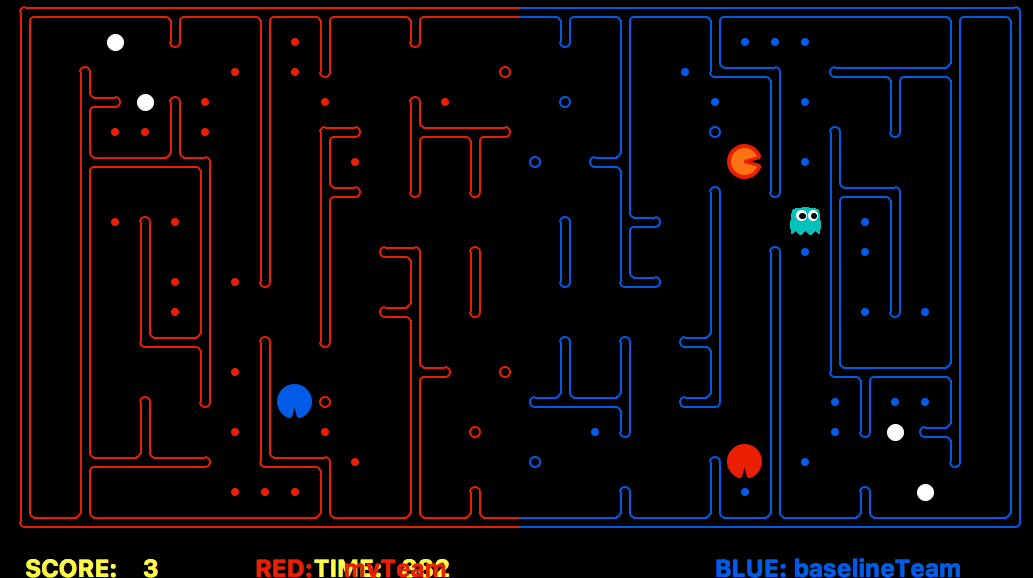
\includegraphics[width=0.5\textwidth]{report_fig1.png}
\caption{\label{fig:1}Map Bottleneck}
\end{wrapfigure}

Most levels had a spot where, the ghost
could stay and completely block the enemy pacman from winning.
If we could teach our agent how to find the natural bottleneck position, then that would
prevent offense from consuming more pellets.
Therefore, our next goal became to model the game level in such a way that
allowed us to find this position given any pacman map layout. \

We chose to model the map as a network flow graph, and use Ford-Fulkerson
to determine the maximum flow in the graph. We constructed a framework that could
convert the given into a flow network, where vertices are the possible
non-wall positions and the edges are ordered pairs of possible positions. We gave two edges
(one forward and one backward) for each pair of adjacent positions. We set the capacities of
all these edges to 1. We then added a source node and attached an edge with capacity
$\infty$\ to each of the vertices next to the middle line \footnote{Please see the \textit{FlowNetwork} object.}.\



After several small modifications to
Ford-Fulkerson and A* we were able
to find the bottleneck position and successfully find a path to its location.
However it became apparent that not all bottleneck locations were created equal.
That is, bottlenecks whose relative positions that were far away from the red-blue
border, were not useful to guard.\

Therefore we needed to find the bottleneck position with the most pacdots behind it in a particular game instance.
For each pacDot, we did the following:
\begin{enumerate}
	\item Find the max flow from the source to the pacDot, and the path through the maze that's returned by that max flow.
	      This flow will block any paths from the source to the given dot
	\item With the max flow still in place, for each vertex in the returned path, do the following:
	\begin{enumerate}
		\item Try to find an augmenting path through the flow using a modified version of A* from the source to the given vertex
		\item If a path exists, that means there's more than one way to get to this vertex, and we continue.\\
		      Otherwise, the vertex is being blocked by the max flow, and there is only one way to get to that vertex. Store this vertex.
	\end{enumerate}
\end{enumerate}
We then end up with a list of all of the bottlenecks for all of the pacDots.
We find the most commonly recurring bottleneck position, and that's the one we decide to go to.
We point our defense agent to that spot and tell him to stay there as long as possible.
\footnote{Please see the \textit{findBottleneckWithMostPacdots(self, gameState)} method on the \textit{DummyAgent} object, which calls
the \textit{FindBottlenecks(self, source, target)} method on the \textit{FlowNetwork} object.}

\section{Final Tweaks and Manual Override}

After implementing a max flow defensive agent and correctly modeling the map as a flow network,
our agent was performing well and placing in $8^{th}$ in the tournaments.
Our focus shifted away from the Q-learing agent and it seemed more practical in the amount of time remaining,
to manually make the pacman avoid negative cases.

\subsection{Eating Pacmen}
Neither of our agents were ever told to eat pacmen, and this was a poor strategy.
We programmed a procedure for both agents, to decide whether it should attack an enemy based on the A* distance from that enemy.
We noticed on offense, if an enemy was an even number of steps away from our agent, it was easy for our agent to avoid the
enemy. For the defense agent, we made sure that the distance between
the agent and the bottleneck is less than the distance between the enemy and the bottleneck.
This allowed the agent to guard the bottleneck while still being able to attack enemies.

\subsection{Avoiding ghosts}
While our Q learning agent had figured out that it should avoid ghosts by itself, it did not avoid ghosts reliably.
We integrated a parameter into out A* search algorithm that gave a very high weight to
all positions with enemy ghosts in them. Therefore the offensive agent would avoid enemy ghosts if possible. \

The offensive agent also trapped itself into corners where the ghost would easily kill it.
We used network flow again to determine if a ghost was nearby.
We checked all nearby pacdots for one that has a maximum flow greater than 1 and therefore
there is more than one path, which created less opportunities to become trapped.
\footnote{Please see the \textit{aStarSearch(self, startPosition, gameState, goalPositions, attackPacmen=True)} method
on the \textit{DummyAgent}.}


\section{Conclusions}
Although we set out to create an overall offensive/defensive agent, separating
offensive and defensive concerns proved to be a valuable strategy. We realized that
narrowing the problem down into smaller subproblems allowed us to focus and perfect
one strategy independent of the other. The results showed that this approach is very
useful when attempting to solve and model large, dynamic environments such as Capture the Flag.


\end{document}
